\chapter{集合と写像}
\section{集合論}
\subsection{集合}
数学において\emph{集合}\index{しゅうごう@集合}(Set)は最も基礎的な概念とも言われており、様々な概念が集合を元に記述される。集合は直感的に分かる通り「何かの集まり」である\footnote{これは直感的ではあるが、数学的にはかなり曖昧な定義である。実は先述のような直感的な集合の定義では矛盾が生じる場合があることが知られている(ラッセルのパラドックス)。これを回避するため、集合という概念そのものを厳密に定義する試みが100年ほど前に公理的集合論という数学上の分野で行われた。その結果、上述の矛盾を引き起こすようなものは「集合ではない」として排除され、クラス(類)という新たな概念に分類される。また、公理的集合論では選択公理と呼ばれる公理が存在し、これを採用する数学理論、採用しない数学理論が展開される。このように集合論の公理的構成は興味深いものではあるが、本文書で扱う部分においては前述の直感的な理解で問題ない。}。集合の要素は数である必要はないし、含まれる要素の個数も有限でなくてもよい。まず、集合における、高校数学までの基礎的な用語の定義を以下にまとめる。
\begin{definition*}{集合の用語}
	\begin{itemize}
		\item 集合\(A\)に集合\(B\)が含まれることを「集合\(B\)は集合\(A\)の\emph{部分集合}である」と言い、\(B \subseteq A\)と書く。
		\item 集合\(A\)の部分集合\(B\)が\(A\)自体を含まない場合、「集合\(B\)は集合\(A\)の\emph{真部分集合}である」と言い、\(B \subset A\)と書く。
		\item 要素\(a\)が集合\(A\)に含まれている場合、「\(a\)は集合\(A\)の\emph{要素}である」と言い、\(a \in A\)と書く。
		\item 要素を一つも持たない集合を\emph{空集合}と呼び、\(\varnothing\)などと表す。
	\end{itemize}
\end{definition*}
ただし、真部分集合と部分集合を同一に扱っている場合もあり、部分集合を\(B \subset A\)と書いてある場合もある。包含関係を示す記号には逆方向(\(\ni \), \(\supseteq\),\(\supset\))なども存在するが意味はこれらは文字を入れ替えただけである。

集合を数式によって表現する方法は二通りあり、まず1つ目は要素を列挙する方法である。この方法では、1から6までの自然数を要素に持つ集合\(A\)は以下のように表現される。
\begin{equation}
	A=\{1,2,3,4,5,6\}
\end{equation}
集合自体には順序という概念が存在しないため、要素の順番を入れ替えて記述してもよい。もう一つの方法は、集合に入る要素の条件を記述する方法で、同じ集合は例えば以下のように表すことができる。
\begin{equation}
	A=\{x|xは整数かつ1\leq x \leq 6\}
\end{equation}
ここで、仕切り記号「\(|\)」の前が要素を示し、後が条件を示す。ただ、上記の方法では日本語が含まれているため、もう少しスマートに記述し
\begin{equation}
	A=\{x|x\in \mathbb{Z} \ \mathrm{and} \  1\leq x \leq 6\}
\end{equation}
とも記述できる。ここで、\(\mathbb{Z}\)は自然数全体の集合を示す。更に、「\(x\)が整数(もしくは実数)である」という条件は頻繁に用いるため、以下のように仕切り記号の前においてもよいことになっている。
\begin{equation}
	A=\{x\in \mathbb{Z} | 1\leq x \leq 6\}
\end{equation}
集合という概念は広く、様々な集合を考えることができるが、特に理工学において重要な集合は前述した自然数全体の集合\(\mathbb{Z}\)、実数全体の集合\(\mathbb{R}\)および複素数全体の集合\(\mathbb{C}\)である。

\begin{figure}[ht]
	\centering
	\tikzset{every picture/.style={line width=0.75pt}} %set default line width to 0.75pt
	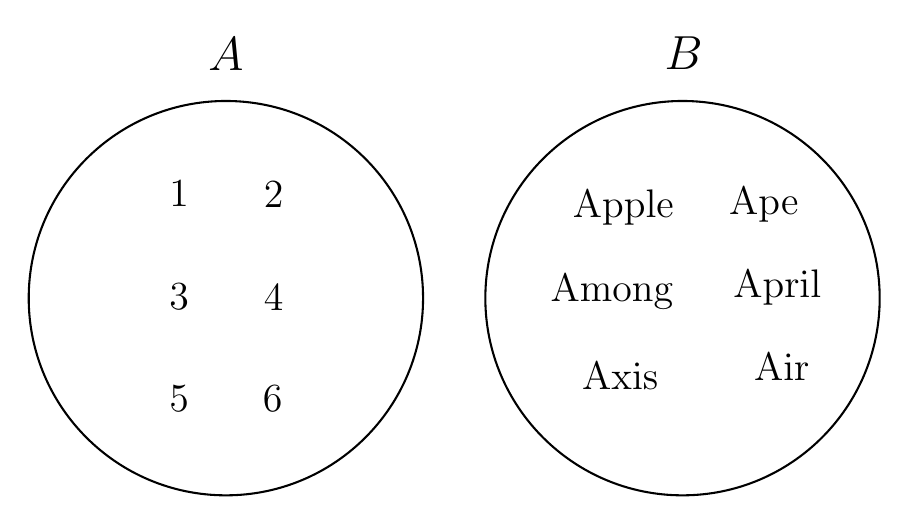
\begin{tikzpicture}[x=0.75pt,y=0.75pt,yscale=-1,xscale=1]
		%uncomment if require: \path (0,438); %set diagram left start at 0, and has height of 438
		%Shape: Circle [id:dp21290940653164325]
		\draw   (70,175) .. controls (70,122.53) and (112.53,80) .. (165,80) .. controls (217.47,80) and (260,122.53) .. (260,175) .. controls (260,227.47) and (217.47,270) .. (165,270) .. controls (112.53,270) and (70,227.47) .. (70,175) -- cycle ;
		%Shape: Circle [id:dp0887475809679914]
		\draw   (290,175) .. controls (290,122.53) and (332.53,80) .. (385,80) .. controls (437.47,80) and (480,122.53) .. (480,175) .. controls (480,227.47) and (437.47,270) .. (385,270) .. controls (332.53,270) and (290,227.47) .. (290,175) -- cycle ;
		% Text Node
		\draw (165.03,57.33) node  [font=\LARGE]  {$A$};
		% Text Node
		\draw (385.5,57) node  [font=\LARGE]  {$B$};
		% Text Node
		\draw (142.5,124.5) node  [font=\Large] [align=left] {1};
		% Text Node
		\draw (188.01,125) node  [font=\Large] [align=left] {2};
		% Text Node
		\draw (142.5,174.5) node  [font=\Large] [align=left] {3};
		% Text Node
		\draw (188.01,175) node  [font=\Large] [align=left] {4};
		% Text Node
		\draw (142.5,223.5) node  [font=\Large] [align=left] {5};
		% Text Node
		\draw (187.5,223.5) node  [font=\Large] [align=left] {6};
		% Text Node
		\draw (356.5,131.5) node  [font=\Large] [align=left] {Apple};
		% Text Node
		\draw (406,120) node [anchor=north west][inner sep=0.75pt]  [font=\Large] [align=left] {Ape};
		% Text Node
		\draw (351,172) node  [font=\Large] [align=left] {Among};
		% Text Node
		\draw (408,160) node [anchor=north west][inner sep=0.75pt]  [font=\Large] [align=left] {April};
		% Text Node
		\draw (355,212.5) node  [font=\Large] [align=left] {Axis};
		% Text Node
		\draw (418,200) node [anchor=north west][inner sep=0.75pt]  [font=\Large] [align=left] {Air};

	\end{tikzpicture}
	\caption{集合の例。集合は要素が数である必要もないし、要素が無限にあってもよい。}
\end{figure}

\subsection{集合の操作}
集合に何らかの操作を行い、新たな集合を作ることはしばしば用いられる操作である。\emph{和集合}\index{わしゅうごう@和集合}(union)および\emph{共通部分}\index{きょうつうぶぶん@共通部分}\footnote{共通部分を積集合と呼ばないのは、後述する直積集合との混乱を避けるためである。intersectionの訳として、交叉集合などとも呼ばれる。}(intersection)は、高校までの数学にあるとおりである。
\begin{definition*}{和集合・共通部分}
	集合\(A\)と集合\(B\)の少なくともどちらか一方に含まれる要素の集合を\emph{和集合}と呼び、\(A \cup B\)と書く。
	\begin{equation}
		A \cup B=\{x| x \in A \ \mathrm{or} \ x \in B\}
	\end{equation}
	同様に、集合\(A\)と集合\(B\)のどちらにも含まれる要素の集合を\emph{共通部分}と呼び、\(A \cap B\)と書く。
	\begin{equation}
		A \cup B=\{x| x \in A \ \mathrm{and} \ x \in B\}
	\end{equation}
\end{definition*}
\(\cup\) はcup、\(\cap\)はcapと呼ばれ、英語で韻を踏んでいる。例えば\(A=\{ 1,2,3,4,5,6\}\)と\(B=\{2,4,6,8,10,12\}\)に対しては
\begin{equation}
	A \cup B=\{1,2,3,4,5,6,8,10,12\}
\end{equation}
\begin{equation}
	A \cap B=\{2,4,6\}
\end{equation}
となる。これらの操作では、自然数の集合と自然数の集合からは同じく自然数の集合が作られるが、更に「自然数のペア」を作ったり、「集合の集合」を作ったりする操作も考えられる。
\emph{冪集合}\index{べきしゅうごう@冪集合}(power set)は、端的に言えば集合\(A\)から要素を取り出す「取り出し方」全ての集合である。
\begin{definition*}{冪集合}
	集合\(A\)の\emph{冪集合}とは集合\(A\)の部分集合全ての集合であり、\(2^A\)などと書く。
	\begin{equation}
		2^A=\{S| S \subseteq A\}
	\end{equation}
\end{definition*}
冪集合においては、\(A\)が要素数\(n\)の有限集合の場合に冪集合の要素数が\(2^n\)になる。例えば\(A=\{1,2,3\}\)の場合、
\begin{equation}
	2^A=\{ \varnothing , \{1\},\{2\}, \{3\}, \{1,2\}, \{1,3\}, \{2,3\}, \{1,2,3\} \}
\end{equation}
のようになる。
これに対し、\emph{直積集合}\index{ちょくせきしゅうごう@直積集合}(Cartesian set)は、集合同士の「ペア」の集合を示す。
\begin{definition*}{直積集合}
	集合\(A\)と集合\(B\)の\emph{直積集合}とは\(A\)と\(B\)の要素ペアの集合であり、\(A\times B\)と表す。
	\begin{equation}
		A \times B=\{(a,b)| a \in A \ \mathrm{and} \ b \in B\}
	\end{equation}
\end{definition*}
直積集合は、例えば\(A=\{1,2,3\}\)、\(B=\{2,4,6\}\)の場合
\begin{equation}
	A \times B=\{(1,2),(1,4),(1,6),(2,2),(2,4),(2,6),(3,2),(3,4),(3,6)\}
\end{equation}
などのように書き下せる。しかし、このような有限集合間の直積集合より、実数集合\(\mathbb{R}\)の直積集合の方が物理的に重要である。なぜなら、3次元空間上の点\((x,y,z)\)は、3つの実数のペアとして表せるため、\(\mathbb{R}\times \mathbb{R}\times \mathbb{R}\)という集合に含まれるためである。このような同じ集合同士の直積集合はよく現れるため、\(\mathbb{R}^3\)などと省略して記述する。
\section{写像}
\subsection{写像と関数}
\emph{写像}\index{しゃぞう@写像}(map)は、集合の要素を結びつける対応関係のことである。写像という概念を説明する方法はいくつかあるが、ここでは「写像とは\emph{関数}\index{かんすう@関数}(function)のことである」と説明する。例えば、中学校や高校で学ぶ関数
\begin{equation}
	f(x)=x^2
\end{equation}
を考える。中学校や高校では明記していないが、一般的にこの関数に与える\(x\)は実数であり、その場合得られる値\(f(x)\)も実数である。これはつまり、関数\(f(x)\)は実数と実数を結びつける対応関係と考えることもできるということを示している。このように関数を写像として捉える時、以下のように表現する。
\begin{equation}
	\begin{aligned}
		f: \mathbb{R}\rightarrow \mathbb{R} \\
		x\longmapsto x^2
	\end{aligned}
\end{equation}
これは、「\(f\)は実数の集合\(\mathbb{R}\)から実数の集合\(\mathbb{R}\)への写像で、元\(x\)が\(x^2\)に写される」という意味である。
\begin{definition*}{写像}
	集合\(A\)から集合\(B\)への\emph{写像}\(f\)は、以下のように表される。
	\begin{equation}
		\begin{aligned}
			f: A\rightarrow B \\
			x\longmapsto f(x)
		\end{aligned}
	\end{equation}
	ここで、\(A\)を\emph{定義域}、\(B\)を\emph{終域}と呼ぶ。また、\(f(x)\)のことを\emph{値}と言い、\(f(x)\)がとり得る値全ての集合を\emph{値域}と呼ぶ。
\end{definition*}
定義域および値域は、高校数学までに関数に対して学んだ用語と同一の意味である。ここで注意すべきなのは、値域と終域が同一であるとは限らないことである。例えば、上記の写像\(f(x)=x^2\)は\(\mathbb{R}\)から\(\mathbb{R}\)への写像であり、その定義域と終域は\(\mathbb{R}\)であるが、値域は\(\mathbb{R}\)ではない。なぜなら得られる値は非負であるため、値域は実数全体のうち非負の部分だけになるためである。この場合、値域は\(\{x\in \mathbb{R}|x\geq0\}\)のように与えられ、\(\mathbb{R}^+\)などのように表現される。

\subsection{全射・単射}
写像はその性質によって全射、単射などと呼ばれる。まず、\emph{単射}\index{たんしゃ@単射}(injective)とは像が重ならないこと、すなわち得られる値に対してその元となった値を必ず1つだけ求められるというものである。
\begin{definition*}{単射}
	定義域を\(A\)、値域を\(B\)としたとき、写像\(f\)が\(A\)に含まれる任意の値\(a_1,a_2(a_1\neq a_2)\)に対して
	\begin{equation}
		\begin{aligned}
			f(a_1)\neq f(a_2)
		\end{aligned}
	\end{equation}
	であるとき、\(f\)が\emph{単射}であると言う。
\end{definition*}
この定義は直感的でないかもしれないが、後に全射とともに図で説明する。
これに対し、\emph{全射}\index{ぜんしゃ@全射}(surjective)の定義は単純で、値域が終域と同一であることを示す。
\begin{definition*}{全射}
	定義域を\(A\)、値域を\(B\)とした写像\(f\)に対し、その値域が終域と一致する時、
	すなわち、任意の\(B\)の要素\(b\)に対し、
	\begin{equation}
		\begin{aligned}
			f(a)= b
		\end{aligned}
	\end{equation}
	となる\(A\)の要素\(a\)が存在する時、\(f\)が\emph{全射}であると言う。
\end{definition*}
全射と単射は重要な性質であるが、対になっているものではない。すなわち、全射であり単射でもある写像というものもあるし、全射でも単射でもない写像もある。このうち、全射かつ単射である写像は集合論において非常に重要であるため、\emph{全単射}\index{ぜんたんしゃ@全単射}(bijective)という名前で呼ばれる。単射・全射について、自然数の集合および実数関数の例を、以下の表に示す。

\begin{figure}[ht]
	\centering

	\begin{tabular}{|c|c|c|}
		\hline
		                               & {全射} & {全射でない} \\
		\hline
		{\raisebox{3.5em}{単射}}       &


		\tikzset{every picture/.style={line width=0.75pt}} %set default line width to 0.75pt

		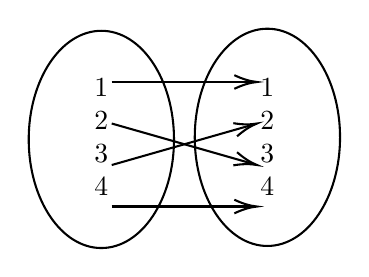
\begin{tikzpicture}[x=0.75pt,y=0.75pt,yscale=-1,xscale=1]
			\centering
			%uncomment if require: \path (0,116); %set diagram left start at 0, and has height of 116

			%Shape: Ellipse [id:dp6412400391115132]
			\draw   (24,60.33) .. controls (24,31.43) and (39.67,8) .. (59,8) .. controls (78.33,8) and (94,31.43) .. (94,60.33) .. controls (94,89.24) and (78.33,112.67) .. (59,112.67) .. controls (39.67,112.67) and (24,89.24) .. (24,60.33) -- cycle ;
			%Shape: Ellipse [id:dp40267433910316797]
			\draw   (104,59.33) .. controls (104,30.43) and (119.67,7) .. (139,7) .. controls (158.33,7) and (174,30.43) .. (174,59.33) .. controls (174,88.24) and (158.33,111.67) .. (139,111.67) .. controls (119.67,111.67) and (104,88.24) .. (104,59.33) -- cycle ;
			%Straight Lines [id:da9087756456779403]
			\draw    (64,32.67) -- (132,32.67) ;
			\draw [shift={(134,32.67)}, rotate = 180] [color={rgb, 255:red, 0; green, 0; blue, 0 }  ][line width=0.75]    (10.93,-3.29) .. controls (6.95,-1.4) and (3.31,-0.3) .. (0,0) .. controls (3.31,0.3) and (6.95,1.4) .. (10.93,3.29)   ;
			%Straight Lines [id:da6700117726346599]
			\draw    (64,52.67) -- (132.08,72.12) ;
			\draw [shift={(134,72.67)}, rotate = 195.95] [color={rgb, 255:red, 0; green, 0; blue, 0 }  ][line width=0.75]    (10.93,-3.29) .. controls (6.95,-1.4) and (3.31,-0.3) .. (0,0) .. controls (3.31,0.3) and (6.95,1.4) .. (10.93,3.29)   ;
			%Straight Lines [id:da5633782208894125]
			\draw    (64,72.67) -- (132.08,53.22) ;
			\draw [shift={(134,52.67)}, rotate = 524.05] [color={rgb, 255:red, 0; green, 0; blue, 0 }  ][line width=0.75]    (10.93,-3.29) .. controls (6.95,-1.4) and (3.31,-0.3) .. (0,0) .. controls (3.31,0.3) and (6.95,1.4) .. (10.93,3.29)   ;
			%Straight Lines [id:da9525525121050697]
			\draw    (64,92.67) -- (132,92.67) ;
			\draw [shift={(134,92.67)}, rotate = 180] [color={rgb, 255:red, 0; green, 0; blue, 0 }  ][line width=0.75]    (10.93,-3.29) .. controls (6.95,-1.4) and (3.31,-0.3) .. (0,0) .. controls (3.31,0.3) and (6.95,1.4) .. (10.93,3.29)   ;

			% Text Node
			\draw (59,60.33) node    {$ \begin{array}{l}
						1 \\
						2 \\
						3 \\
						4
					\end{array}$};
			% Text Node
			\draw (139,60.33) node    {$ \begin{array}{l}
						1 \\
						2 \\
						3 \\
						4
					\end{array}$};


		\end{tikzpicture}
		                               &


		\tikzset{every picture/.style={line width=0.75pt}} %set default line width to 0.75pt

		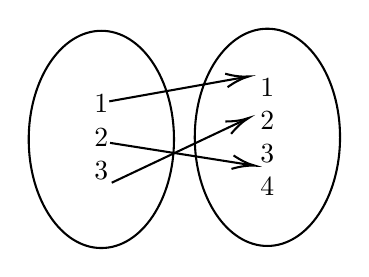
\begin{tikzpicture}[x=0.75pt,y=0.75pt,yscale=-1,xscale=1]
			%uncomment if require: \path (0,116); %set diagram left start at 0, and has height of 116
			\centering
			%Shape: Ellipse [id:dp0034386056158046685]
			\draw   (24,60.33) .. controls (24,31.43) and (39.67,8) .. (59,8) .. controls (78.33,8) and (94,31.43) .. (94,60.33) .. controls (94,89.24) and (78.33,112.67) .. (59,112.67) .. controls (39.67,112.67) and (24,89.24) .. (24,60.33) -- cycle ;
			%Shape: Ellipse [id:dp7088458776496958]
			\draw   (104,59.33) .. controls (104,30.43) and (119.67,7) .. (139,7) .. controls (158.33,7) and (174,30.43) .. (174,59.33) .. controls (174,88.24) and (158.33,111.67) .. (139,111.67) .. controls (119.67,111.67) and (104,88.24) .. (104,59.33) -- cycle ;
			%Straight Lines [id:da22675878536246064]
			\draw    (62.8,42) -- (128.03,30.35) ;
			\draw [shift={(130,30)}, rotate = 529.88] [color={rgb, 255:red, 0; green, 0; blue, 0 }  ][line width=0.75]    (10.93,-3.29) .. controls (6.95,-1.4) and (3.31,-0.3) .. (0,0) .. controls (3.31,0.3) and (6.95,1.4) .. (10.93,3.29)   ;
			%Straight Lines [id:da6109519093828262]
			\draw    (63.2,62) -- (131.02,72.69) ;
			\draw [shift={(133,73)}, rotate = 188.96] [color={rgb, 255:red, 0; green, 0; blue, 0 }  ][line width=0.75]    (10.93,-3.29) .. controls (6.95,-1.4) and (3.31,-0.3) .. (0,0) .. controls (3.31,0.3) and (6.95,1.4) .. (10.93,3.29)   ;
			%Straight Lines [id:da9176125882722679]
			\draw    (64,81.2) -- (128.19,50.85) ;
			\draw [shift={(130,50)}, rotate = 514.7] [color={rgb, 255:red, 0; green, 0; blue, 0 }  ][line width=0.75]    (10.93,-3.29) .. controls (6.95,-1.4) and (3.31,-0.3) .. (0,0) .. controls (3.31,0.3) and (6.95,1.4) .. (10.93,3.29)   ;

			% Text Node
			\draw (59,60.33) node    {$ \begin{array}{l}
						1 \\
						2 \\
						3
					\end{array}$};
			% Text Node
			\draw (139,60.33) node    {$ \begin{array}{l}
						1 \\
						2 \\
						3 \\
						4
					\end{array}$};


		\end{tikzpicture}
		\\
		\hline
		{\raisebox{3.5em}{単射でない}} &


		\tikzset{every picture/.style={line width=0.75pt}} %set default line width to 0.75pt

		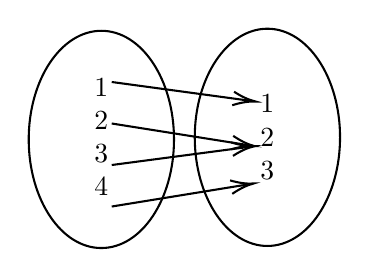
\begin{tikzpicture}[x=0.75pt,y=0.75pt,yscale=-1,xscale=1]
			%uncomment if require: \path (0,116); %set diagram left start at 0, and has height of 116
			\centering
			%Shape: Ellipse [id:dp6129036964567098]
			\draw   (24,60.33) .. controls (24,31.43) and (39.67,8) .. (59,8) .. controls (78.33,8) and (94,31.43) .. (94,60.33) .. controls (94,89.24) and (78.33,112.67) .. (59,112.67) .. controls (39.67,112.67) and (24,89.24) .. (24,60.33) -- cycle ;
			%Shape: Ellipse [id:dp43107862422073095]
			\draw   (104,59.33) .. controls (104,30.43) and (119.67,7) .. (139,7) .. controls (158.33,7) and (174,30.43) .. (174,59.33) .. controls (174,88.24) and (158.33,111.67) .. (139,111.67) .. controls (119.67,111.67) and (104,88.24) .. (104,59.33) -- cycle ;
			%Straight Lines [id:da4221103930385579]
			\draw    (64,32.67) -- (131.35,41.81) ;
			\draw [shift={(133.33,42.08)}, rotate = 187.73] [color={rgb, 255:red, 0; green, 0; blue, 0 }  ][line width=0.75]    (10.93,-3.29) .. controls (6.95,-1.4) and (3.31,-0.3) .. (0,0) .. controls (3.31,0.3) and (6.95,1.4) .. (10.93,3.29)   ;
			%Straight Lines [id:da3750145893222052]
			\draw    (64,52.67) -- (130.86,63.27) ;
			\draw [shift={(132.83,63.58)}, rotate = 189.01] [color={rgb, 255:red, 0; green, 0; blue, 0 }  ][line width=0.75]    (10.93,-3.29) .. controls (6.95,-1.4) and (3.31,-0.3) .. (0,0) .. controls (3.31,0.3) and (6.95,1.4) .. (10.93,3.29)   ;
			%Straight Lines [id:da9480623000921049]
			\draw    (64,72.67) -- (130.85,63.84) ;
			\draw [shift={(132.83,63.58)}, rotate = 532.48] [color={rgb, 255:red, 0; green, 0; blue, 0 }  ][line width=0.75]    (10.93,-3.29) .. controls (6.95,-1.4) and (3.31,-0.3) .. (0,0) .. controls (3.31,0.3) and (6.95,1.4) .. (10.93,3.29)   ;
			%Straight Lines [id:da9582825190855755]
			\draw    (64,92.67) -- (130.36,81.9) ;
			\draw [shift={(132.33,81.58)}, rotate = 530.79] [color={rgb, 255:red, 0; green, 0; blue, 0 }  ][line width=0.75]    (10.93,-3.29) .. controls (6.95,-1.4) and (3.31,-0.3) .. (0,0) .. controls (3.31,0.3) and (6.95,1.4) .. (10.93,3.29)   ;

			% Text Node
			\draw (59,60.33) node    {$ \begin{array}{l}
						1 \\
						2 \\
						3 \\
						4
					\end{array}$};
			% Text Node
			\draw (139,60.33) node    {$ \begin{array}{l}
						1 \\
						2 \\
						3
					\end{array}$};


		\end{tikzpicture}
		                               &


		\tikzset{every picture/.style={line width=0.75pt}} %set default line width to 0.75pt

		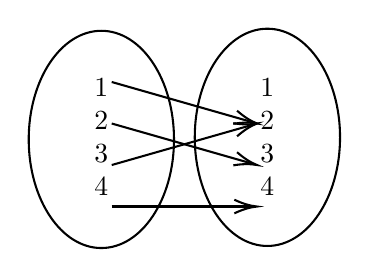
\begin{tikzpicture}[x=0.75pt,y=0.75pt,yscale=-1,xscale=1]
			%uncomment if require: \path (0,116); %set diagram left start at 0, and has height of 116
			\centering
			%Shape: Ellipse [id:dp8960685448671817]
			\draw   (24,60.33) .. controls (24,31.43) and (39.67,8) .. (59,8) .. controls (78.33,8) and (94,31.43) .. (94,60.33) .. controls (94,89.24) and (78.33,112.67) .. (59,112.67) .. controls (39.67,112.67) and (24,89.24) .. (24,60.33) -- cycle ;
			%Shape: Ellipse [id:dp857197083920707]
			\draw   (104,59.33) .. controls (104,30.43) and (119.67,7) .. (139,7) .. controls (158.33,7) and (174,30.43) .. (174,59.33) .. controls (174,88.24) and (158.33,111.67) .. (139,111.67) .. controls (119.67,111.67) and (104,88.24) .. (104,59.33) -- cycle ;
			%Straight Lines [id:da6439600711736742]
			\draw    (64,32.67) -- (132.08,52.12) ;
			\draw [shift={(134,52.67)}, rotate = 195.95] [color={rgb, 255:red, 0; green, 0; blue, 0 }  ][line width=0.75]    (10.93,-3.29) .. controls (6.95,-1.4) and (3.31,-0.3) .. (0,0) .. controls (3.31,0.3) and (6.95,1.4) .. (10.93,3.29)   ;
			%Straight Lines [id:da002958833898464963]
			\draw    (64,52.67) -- (132.08,72.12) ;
			\draw [shift={(134,72.67)}, rotate = 195.95] [color={rgb, 255:red, 0; green, 0; blue, 0 }  ][line width=0.75]    (10.93,-3.29) .. controls (6.95,-1.4) and (3.31,-0.3) .. (0,0) .. controls (3.31,0.3) and (6.95,1.4) .. (10.93,3.29)   ;
			%Straight Lines [id:da7886515175891524]
			\draw    (64,72.67) -- (132.08,53.22) ;
			\draw [shift={(134,52.67)}, rotate = 524.05] [color={rgb, 255:red, 0; green, 0; blue, 0 }  ][line width=0.75]    (10.93,-3.29) .. controls (6.95,-1.4) and (3.31,-0.3) .. (0,0) .. controls (3.31,0.3) and (6.95,1.4) .. (10.93,3.29)   ;
			%Straight Lines [id:da8765014602231163]
			\draw    (64,92.67) -- (132,92.67) ;
			\draw [shift={(134,92.67)}, rotate = 180] [color={rgb, 255:red, 0; green, 0; blue, 0 }  ][line width=0.75]    (10.93,-3.29) .. controls (6.95,-1.4) and (3.31,-0.3) .. (0,0) .. controls (3.31,0.3) and (6.95,1.4) .. (10.93,3.29)   ;

			% Text Node
			\draw (59,60.33) node    {$ \begin{array}{l}
						1 \\
						2 \\
						3 \\
						4
					\end{array}$};
			% Text Node
			\draw (139,60.33) node    {$ \begin{array}{l}
						1 \\
						2 \\
						3 \\
						4
					\end{array}$};


		\end{tikzpicture}
		\\
		\hline
	\end{tabular}
	\caption{数個の自然数による集合における全射・単射の例}
\end{figure}

\begin{figure}[H]
	\centering

	\begin{tabular}{|c|c|c|}
		\hline
		           & 全射                                      & 全射でない \\
		\hline
		単射       & \makecell[c]{$\displaystyle f( x) =2x+1$               \\
			\tikzset{every picture/.style={line width=0.75pt}} %set default line width to 0.75pt
			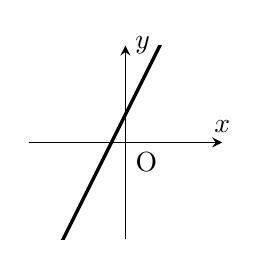
\begin{tikzpicture}[x=10pt,y=10pt,yscale=1,xscale=1]
				\draw[->,>=stealth,semithick] (-3.5,0)--(3.5,0)node[above]{$x$}; %x軸
				\draw[->,>=stealth,semithick] (0,-3.5)--(0,3.5)node[right]{$y$}; %y軸
				\draw (0,0)node[below right]{O}; %原点
				\begin{scope} \clip (-3.5,-3.5) rectangle (3.5,3.5);
					\draw[very thick,,samples=5,domain=-3.5:3.5] plot(\x,2*\x+1);
				\end{scope}
			\end{tikzpicture}
		}
		           & \makecell[c]{$\displaystyle f( x) =e^x$                \\
			\tikzset{every picture/.style={line width=0.75pt}} %set default line width to 0.75pt
			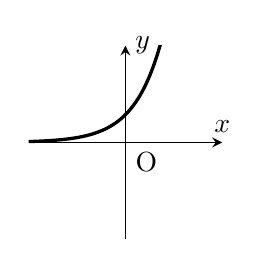
\begin{tikzpicture}[x=10pt,y=10pt,yscale=1,xscale=1]
				\draw[->,>=stealth,semithick] (-3.5,0)--(3.5,0)node[above]{$x$}; %x軸
				\draw[->,>=stealth,semithick] (0,-3.5)--(0,3.5)node[right]{$y$}; %y軸
				\draw (0,0)node[below right]{O}; %原点
				\begin{scope} \clip (-3.5,-3.5) rectangle (3.5,3.5);
					\draw[very thick,,samples=100,domain=-3.5:3.5] plot(\x,exp{(\x)});
				\end{scope}
			\end{tikzpicture}
		}
		\\
		\hline
		単射でない & \makecell[c]{$\displaystyle f( x) =x^3-x$              \\
			\tikzset{every picture/.style={line width=0.75pt}} %set default line width to 0.75pt
			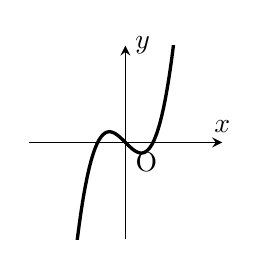
\begin{tikzpicture}[x=10pt,y=10pt,yscale=1,xscale=1]
				\draw[->,>=stealth,semithick] (-3.5,0)--(3.5,0)node[above]{$x$}; %x軸
				\draw[->,>=stealth,semithick] (0,-3.5)--(0,3.5)node[right]{$y$}; %y軸
				\draw (0,0)node[below right]{O}; %原点
				\begin{scope} \clip (-3.5,-3.5) rectangle (3.5,3.5);
					\draw[very thick,,samples=100,domain=-3.5:3.5] plot(\x,\x^3-\x);
				\end{scope}
			\end{tikzpicture}
		}
		           & \makecell[c]{$\displaystyle f( x) =x^2$                \\
			\tikzset{every picture/.style={line width=0.75pt}} %set default line width to 0.75pt
			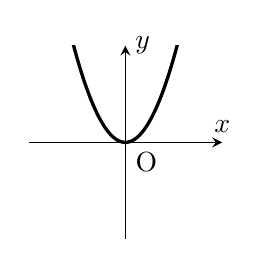
\begin{tikzpicture}[x=10pt,y=10pt,yscale=1,xscale=1]
				\draw[->,>=stealth,semithick] (-3.5,0)--(3.5,0)node[above]{$x$}; %x軸
				\draw[->,>=stealth,semithick] (0,-3.5)--(0,3.5)node[right]{$y$}; %y軸
				\draw (0,0)node[below right]{O}; %原点
				\begin{scope} \clip (-3.5,-3.5) rectangle (3.5,3.5);
					\draw[very thick,,samples=100,domain=-3.5:3.5] plot(\x,\x*\x);
				\end{scope}
			\end{tikzpicture}
		}
		\\
		\hline
	\end{tabular}
	\caption{実数関数における単射・全射の例。
		ここでは定義域および終域を\(\mathbb{R}\)とした。このような \(\mathbb{R}\rightarrow \mathbb{R}\)の実数関数の場合、横に引いた線と関数の交点数が0の部分があるなら全射ではなく、2つ以上の部分があるなら単射ではない。}
\end{figure}

\subsection{多変数関数・多価関数}
以下では実数の集合\(\mathbb{R}\)内での写像(関数)を主に扱う。ここまでの関数は1つの実数を受け取り1つの実数を出す関数であった。これに対して、本文書では受け取る値や出す値が2つ以上存在する場合もある。\emph{多変数関数}\index{たへんすうかんすう@多変数関数}は受け取る値(変数)が複数ある関数である。
\begin{definition*}{多変数関数}
	\(n\)個の変数\(x_1,x_2,...x_n\)を受け取る関数(\(n\geq 2\))を\emph{多変数関数}と呼ぶ。この時、「\(n\)個の実数を受け取り1つの実数を返す関数\(f\)」を
	\begin{equation}
		\begin{aligned}
			f: \mathbb{R}^n\rightarrow \mathbb{R} \\
		\end{aligned}
	\end{equation}
	のように表現し、\(f\)の持つ変数を明示する際には
	\begin{equation}
		\begin{aligned}
			f(x_1,x_2,...x_n)
		\end{aligned}
	\end{equation}
	と表記する。
\end{definition*}
このような多変数関数は、物理的にはよく現れる。例えば3次元空間上の各点におけるなんらかの値を\(f(x,y,z)\)などと記述することは非常に多い。このような場合、ベクトル\(\boldsymbol{v}=(x,y,z)\)を用いて関数を\(f(\boldsymbol{v})\)と記述することもできる(ベクトルについては後述する)。
逆に、複数の値を返す関数もあり、これは\emph{多価関数}\index{たかかんすう@多価関数}と呼ばれる。多価関数は、厳密には関数ではないと考えられる場合もある。なぜなら変数の値を決めても返す値が1つに定まらないためである。ただし、これらの値をペアとして(直積集合として)並べることで、関数のように表現できる。
\begin{definition*}{多価関数}
	\(n\)個の数\(x_1,x_2,...x_n\)を返す関数(\(n\geq 2\))を\emph{多価関数}と呼ぶ。この関数\(f\)は
	\begin{equation}
		\begin{aligned}
			f: \mathbb{R}\rightarrow \mathbb{R}^n \\
		\end{aligned}
	\end{equation}
	のように表現し、\(f\)の返す値を並べて
	\begin{equation}
		\begin{aligned}
			f(x)=(y_1,y_2,...,y_n)
		\end{aligned}
	\end{equation}
	などと表記することもできる。
\end{definition*}
多価関数は、例えば三角関数の逆関数
\begin{equation}
	\begin{aligned}
		f(x)=\sin^{-1}{x}
	\end{aligned}
\end{equation}
などが考えられる。これは、\(x=0\)の際に
\begin{equation}
	\begin{aligned}
		f(0)=(... -2\pi, \pi, 0, \pi, 2\pi, ...)
	\end{aligned}
\end{equation}
となるように、無限個の値をとる多価関数である。ただ、本文書で扱う内容としてはこのような形の多価関数よりも、ベクトル値を返すという意味での多価関数が重要である。例えば、3次元空間上の点\(\boldsymbol{p}=(x,y,z)\)における速度を表す関数\(f(\boldsymbol{p})\)は速度ベクトル\(\boldsymbol{u}=(u,v,w)\)を返す多変数・多価関数である。すなわち、\(f(\boldsymbol{p})\)自体がベクトルであるので、これを表すために\(f\)を太字にして以下のようにも表すことができる。
\begin{definition*}{3次元空間上の多変数・多価関数}
	3次元空間上のベクトル\(\boldsymbol{p}=(x,y,z)\)を変数とし、ベクトル\(\boldsymbol{u}=(u,v,w)\)を返す関数は、3変数、3価の関数で、
	\begin{equation}
		\begin{aligned}
			f: \mathbb{R}^3\rightarrow \mathbb{R}^3 \\
			\boldsymbol{f}(\boldsymbol{p})=\boldsymbol{u}
		\end{aligned}
	\end{equation}
	のように表すことができる。これは1つのベクトルを変数に、1つのベクトルを返す関数とも考えられる。
\end{definition*}
このようなベクトルを得たり、ベクトルを返したりする関数は物理学上非常によく現れる。特に本文書ではテンソルの導入に使用する。
